%!TEX program = xelatex
% Note: this template must be compiled with XeLaTeX rather than PDFLaTeX
% due to the custom fonts used.

\documentclass[
  aspectratio=169,
  t,
  onlytextwidth,
  10pt,
]{beamer}

\usepackage{../../ImperialTheme/beamer/beamerthemeImperial}
\usepackage{xcolor}
\usepackage{amsmath}
\usepackage{multirow}
\usepackage{booktabs}

\def\imagefolder{../../ImperialTheme/beamer/Images}
\def\Rey{\text{Re}}
\newcommand{\qb}{\bar{q}}
\newcommand{\PhiT}{\Phi_T}

\title{Compressible direct linear solver and impulse-response statistics}

\author{Víctor Ballester and Claude}

\date{26 October 2026}

\begin{document}

\begingroup
\setbeamercolor{background canvas}{bg=ICLLightGrey}
\setbeamercolor{title page title}{fg=ICLBlue}
\setbeamercolor{title page subtitle}{fg=ICLBlue}
\setbeamercolor{author}{fg=ICLBlue}
\setbeamercolor{date}{fg=ICLBlue}
\setbeamertemplate{title page}[logo]{\imagefolder/ICL_Logo_Blue.pdf}
\frame[plain, s]{\titlepage}
\endgroup

%----------------------------------------------------------------------
\begin{frame}
	\frametitle{Goal and idea}
	\begin{itemize}
		\item Last time: eigenmodes of the linear operator with Arnoldi, the operator applied by finite differences of the \emph{nonlinear} time stepper (no linearised compressible equations needed).
		\item Now: \textbf{integrate the linear problem in time} (direct linear solver, like \texttt{EvolutionOperator = Direct} of the incompressible solver), still using only the nonlinear time stepper $\PhiT$:
		      \[
			      q'_{k+1} = \frac{\PhiT(\qb + \epsilon_k q'_k) - \PhiT(\qb)}{\epsilon_k},
		      \]
		      period by period ($T$ = rescaling period), with $\epsilon_k$ reset from $\|q'_k\|$ every period, so that the perturbation stays linear however much it grows.
		\item The session is that of the \textbf{nonlinear problem}: nonlinear boundary conditions, sponges, implicit DIRK2, the DNS steady state as \texttt{BaseFlow}. The perturbation boundary conditions follow from the nonlinear ones.
		\item Goal: fast, converged $\overline{u'u'}$, $\overline{u'v'}$, $\overline{v'v'}$ for all the compressible gaps (Ma 0.05--0.8).
	\end{itemize}
\end{frame}

%----------------------------------------------------------------------
\begin{frame}
	\frametitle{Implementation in Nektar++ (\texttt{Driver = JacobianFreeDirect})}
	\small
	\begin{itemize}
		\item New driver deriving from \texttt{DriverArnoldi}; it reuses the Jacobian-free set-up of the Arnoldi drivers:
		      \begin{itemize}\footnotesize
			      \item $\PhiT(\qb)$ is evolved once and cached (\texttt{baseflow\_evolved.fld}), so a base flow that is not an exact discrete steady state does not pollute the difference;
			      \item checkpoints contain the perturbation, including the \emph{linearised} $u'$, $v'$, $p'$ (\texttt{OutputExtraFields}), computed by the same finite difference.
		      \end{itemize}
		\item Perturbation forcing: \texttt{<FORCE TYPE="Field" PERTURBATION="True">} is scaled by $\epsilon_k$ in the perturbed run and switched off in the base-flow run, so it drives $q'$ unscaled. Other forcings (sponge) stay part of the nonlinear operator.
		\item Random forcing (\texttt{awgn}) is evaluated once per time level, so it is the same in all the Newton iterations of a DIRK stage.
		\item Statistics accumulated by the driver itself (filters would see $\qb + \epsilon q'$): means and products $uu$, $uv$, $vv$, $pp$, written like the Reynolds-stresses filter (\texttt{InitialTime}, \texttt{FinalTime}, \texttt{NumberOfFieldDumps}).
		\item Regression test (forced compressible channel): matches an independent small-amplitude nonlinear DNS to 5--6 significant digits, independently of the rescaling period.
	\end{itemize}
\end{frame}

%----------------------------------------------------------------------
\begin{frame}
	\frametitle{What went wrong on the way (and the fixes)}
	\small
	\begin{itemize}
		\item \textbf{Size of the perturbation at low Mach.} $\epsilon$ is set from the global norm, dominated by $E\approx714$ at Ma 0.05, and the packet is local and grows $\sim25\times$ over the gap \emph{within} a period: the gap amplification saturated (nonlinear). Fix: shorter rescaling period.
		      \begin{center}\footnotesize
			      \begin{tabular}{ccc}
				      \toprule
				      $\delta$ ($\epsilon\|q'\|=\delta(1+\|\qb\|)$) & $\|q'\|$ at $t=294$, $T=98$ & $\|q'\|$ at $t=294$, $T=24.5$ \\
				      \midrule
				      $10^{-5}$          & 569 & 915 \\
				      $3\times10^{-6}$   & 606 & 742 \\
				      $10^{-6}$          & 692 & 744 \\
				      $3\times10^{-7}$   & 737 & 752 \\
				      \bottomrule
			      \end{tabular}
		      \end{center}
		\item \textbf{Rounding floor of Newton at large $\Delta t$ and small $\delta$} (pressure $\sim570\times$ the dynamic pressure at Ma 0.05): $\delta=10^{-6}$ with $T=98$, $\Delta t=0.5$ was 85\% off.
		\item \textbf{Under-resolved forcing}: the dipole of the incompressible study (\texttt{weight} = 100, width 0.07) falls on 1--2 quadrature points (spacing $\sim0.9$): the receptivity depends on mesh and discretisation. Resolved dipole (\texttt{weight} = 1, width 0.7) used for the comparisons.
		\item The forcing at $x_0=-95$ lies inside the inlet sponge ($-100<x<-75$, damping $\sim e^{-15}$): inlet sponge switched off.
	\end{itemize}
\end{frame}

%----------------------------------------------------------------------
\begin{frame}
	\frametitle{Time step: large $\Delta t$ is fine (but not that cheap)}
	\small
	\begin{columns}[T]
		\begin{column}{0.52\linewidth}
			\centering\footnotesize
			\renewcommand{\arraystretch}{1.15}
			\begin{tabular}{ccc}
				\toprule
				$\Delta t$ & difference in $u'$, $v'$ & cost per time unit \\
				           & vs $\Delta t=0.007$       & (relative) \\
				\midrule
				0.007 & --                    & 1 \\
				0.1   & $<0.1\%$              & $\sim1/3$ \\
				0.2   & $<0.3\%$ (Ma 0.2, 0.4) & $\sim1/4$ \\
				0.5   & 0.3--2\% (9\% $v'$ over the gap) & $\sim1/4.5$ \\
				\bottomrule
			\end{tabular}
		\end{column}
		\begin{column}{0.46\linewidth}
			\begin{itemize}\footnotesize
				\item DIRK2 damping/phase error at the TS frequencies ($\omega\lesssim0.3$) is negligible up to $\Delta t\approx0.5$.
				\item The saving is smaller than the $\Delta t$ ratio: Newton needs many more iterations per step at large $\Delta t$.
				\item Impulse runs: $\Delta t=0.2$ vs $0.007$ for $\int u'^2dt$, $\int u'v'dt$, $\int v'^2dt$: $4$--$5\times10^{-4}$.
				\item \textbf{$\Delta t = 0.2$} for the batch.
			\end{itemize}
		\end{column}
	\end{columns}
\end{frame}

%----------------------------------------------------------------------
\begin{frame}
	\frametitle{Validation against the incompressible linear solver (Ma 0.05)}
	\begin{columns}[T]
		\begin{column}{0.62\linewidth}
			\centering
			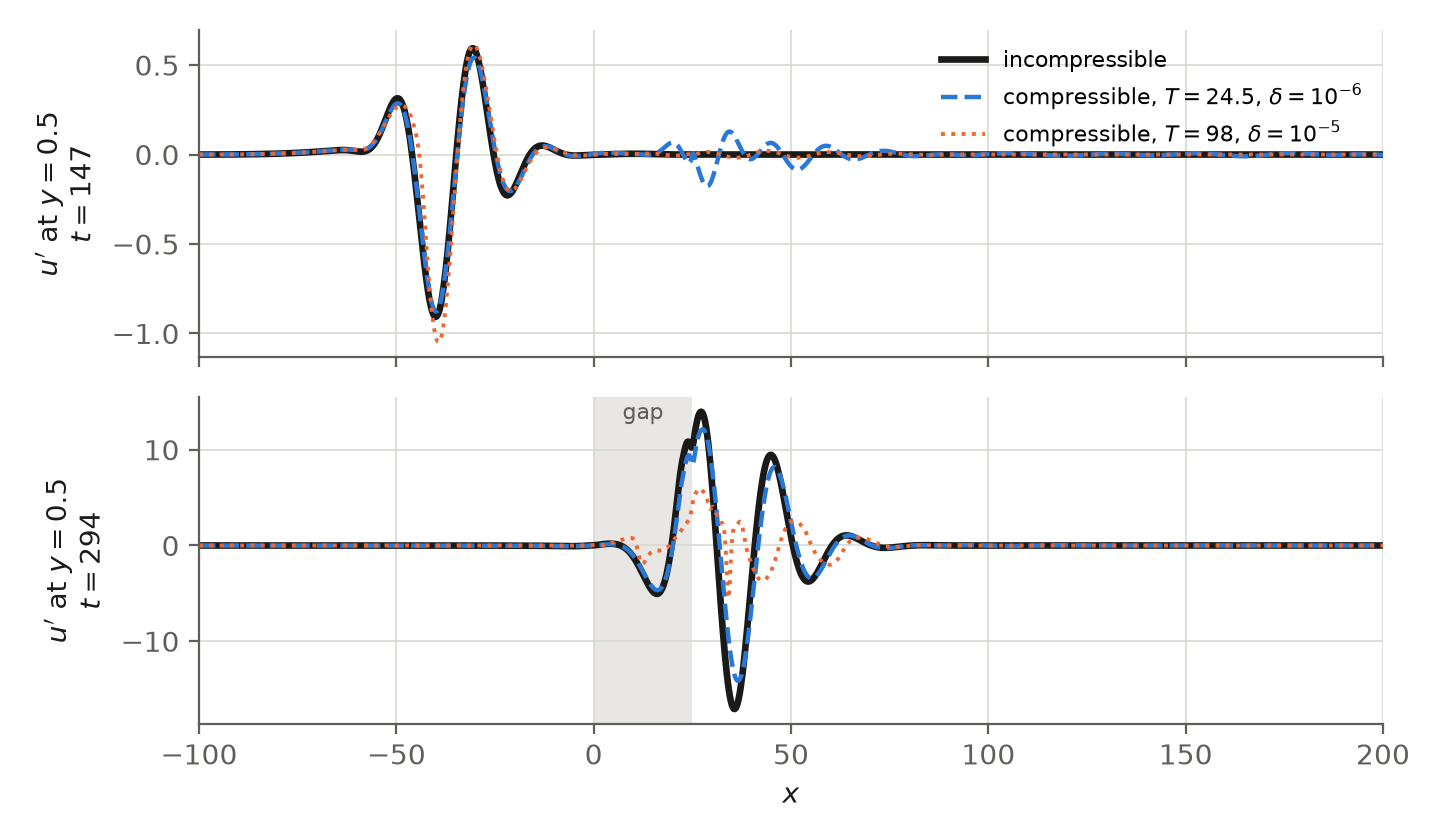
\includegraphics[width=\linewidth]{Images/pulse_fix.png}
		\end{column}
		\begin{column}{0.36\linewidth}
			\footnotesize
			\begin{itemize}
				\item Same mesh (incompressible case), same base flow (incompressible one in conservative variables), resolved dipole, Gaussian pulse in time.
				\item Upstream and through the gap: amplitudes within 2--3\%; downstream of the gap within 17\%.
				\item Before the fix ($T=98$): the gap amplification was $3\times$ too small (nonlinear saturation).
				\item The small waves ahead of the packet ($t=147$) are acoustic, absent in the incompressible solver.
			\end{itemize}
		\end{column}
	\end{columns}
\end{frame}

%----------------------------------------------------------------------
\begin{frame}
	\frametitle{Statistics from one run: the impulse response}
	\small
	Linear system forced by white noise in time with a fixed spatial shape $b$ (the dipole):
	\[
		\frac{dq'}{dt} = \mathcal{L}q' + b\,\xi(t),\qquad \langle\xi(t)\xi(t')\rangle=\sigma^2\delta(t-t')
		\quad\Rightarrow\quad q'(t)=\int_{-\infty}^{t}e^{\mathcal{L}(t-s)}\,b\,\xi(s)\,ds .
	\]
	With the impulse response $q_{\rm imp}(\tau)=e^{\mathcal{L}\tau}b$ (initial condition $b$, no forcing):
	\[
		\langle q'q'^{T}\rangle = \sigma^2\int_0^{\infty} q_{\rm imp}(\tau)\,q_{\rm imp}^T(\tau)\,d\tau
		\quad\Big(\Leftrightarrow\ \mathcal{L}C + C\mathcal{L}^T + \sigma^2 bb^T = 0\Big),
	\]
	so $\overline{u'u'}(x,y)=\sigma^2\int_0^\infty u_{\rm imp}^2\,d\tau$, \ $\overline{u'v'}=\sigma^2\int_0^\infty u_{\rm imp}v_{\rm imp}\,d\tau$, \dots
	\begin{itemize}
		\item One deterministic run per case, until the packet has left the domain ($t\approx3600$): no statistical noise, no averaging window. The driver statistics give the integrals (mean $\times$ run time).
		\item Requires a globally stable flow (otherwise a noise run never becomes stationary either).
		\item Model: a coherent dipole driven by one white-noise signal. The \texttt{awgn} per quadrature point of the incompressible study is spatially white noise (one source per point): not reducible to one run, and mesh dependent.
	\end{itemize}
\end{frame}

%======================================================================
% Detailed comparison: white-noise run vs impulse run
%======================================================================
\begin{frame}
	\frametitle{Noise run vs impulse run: what each one computes}
	\footnotesize
	\renewcommand{\arraystretch}{1.25}
	\begin{tabular}{p{0.2\linewidth}p{0.37\linewidth}p{0.37\linewidth}}
		\toprule
		& \textbf{White-noise run} (incompressible study) & \textbf{Impulse run} (new) \\
		\midrule
		Equation & $\dot q = \mathcal{L}q + b\,\xi(t)$, \ $\xi$ random, new value every step & $\dot q = \mathcal{L}q$, \ no forcing \\
		Initial condition & anything (forgotten after a transient) & $q(0)=b$ (the forcing shape) \\
		Output & time average $\frac{1}{T_{avg}}\int_{t_0}^{t_0+T_{avg}} q\,q^T dt$ & time integral $\int_0^{\infty} q\,q^T dt$ \\
		Estimates & $C=\langle q q^T\rangle$ (ensemble average over the noise) & $C/\sigma^2$, \emph{exactly} \\
		Error & statistical: $\sim\sqrt{2\tau_c/T_{avg}}$ ($\tau_c$: correlation time), plus transient & round-off (the integral is converged once the packet has left) \\
		Length & transient + long $T_{avg}$ (inc.\ study: 24000) & until the packet leaves the domain ($\sim$3600) \\
		Valid for & any forcing statistics & forcing $= $ fixed shape $\times$ one white-noise signal (rank 1), \\
		& & or one run per independent source \\
		\bottomrule
	\end{tabular}
	\vspace{0.2cm}

	\small Both need: linear dynamics, a globally stable flow (otherwise there is no stationary state), zero-mean noise.
\end{frame}

%----------------------------------------------------------------------
\begin{frame}
	\frametitle{Equivalence, step by step (continuous time)}
	\small
	\textbf{1. Response to the forcing.} $\dot q=\mathcal{L}q+b\,\xi(t)$, started long ago, is the convolution with the impulse response $h(\tau)=e^{\mathcal{L}\tau}b$:
	\[
		q(t)=\int_{-\infty}^{t} e^{\mathcal{L}(t-s)}\,b\,\xi(s)\,ds=\int_0^\infty h(\tau)\,\xi(t-\tau)\,d\tau .
	\]
	\textbf{2. Average over the noise} (ensemble average at fixed $t$), using $\langle\xi(s)\,\xi(s')\rangle=\sigma^2\delta(s-s')$:
	\[
		\langle q(t)\,q(t)^T\rangle=\int_0^\infty\!\!\int_0^\infty h(\tau)\,h(\tau')^T\,\underbrace{\langle\xi(t-\tau)\,\xi(t-\tau')\rangle}_{\sigma^2\delta(\tau-\tau')}\,d\tau\,d\tau'
		=\sigma^2\int_0^\infty h(\tau)\,h(\tau)^T\,d\tau .
	\]
	The $\delta$ kills the double integral: different instants of white noise are uncorrelated, so each past kick contributes its own $h\,h^T$ and the cross terms vanish on average.

	\textbf{3. The result does not depend on $t$} (stationary response); $C$ also solves $\mathcal{L}C+C\mathcal{L}^T+\sigma^2bb^T=0$ (Lyapunov).

	\textbf{4. Pointwise,} the diagonal and the off-diagonal blocks give all the Reynolds stresses:
	\[
		\overline{u'u'}(\mathbf{x})=\sigma^2\!\int_0^\infty u_h(\mathbf{x},\tau)^2d\tau,\quad
		\overline{u'v'}(\mathbf{x})=\sigma^2\!\int_0^\infty u_h v_h\,d\tau,\quad
		\overline{v'v'}=\sigma^2\!\int_0^\infty v_h^2\,d\tau,\ \dots
	\]
\end{frame}

%----------------------------------------------------------------------
\begin{frame}
	\frametitle{Why the time average of the noise run gives the same $C$}
	\small
	\begin{itemize}
		\item Step 2 is an \emph{ensemble} average: many independent noise realisations, at one instant. The noise run gives a \emph{time} average of one realisation.
		\item For a stable linear system driven by stationary noise, $q(t)$ is stationary and ergodic: the time average converges to the ensemble average,
		      \[
			      \frac{1}{T_{avg}}\int_{t_0}^{t_0+T_{avg}} q\,q^T dt \ \xrightarrow{\ T_{avg}\to\infty\ }\ C ,
		      \]
		      but only as fast as independent samples accumulate: relative error $\sim\sqrt{2\tau_c/T_{avg}}$, with $\tau_c$ the correlation time of $q\,q^T$ (here: a wavepacket transit time, $O(10^2$--$10^3)$).
		\item The impulse run evaluates the integral of step 2 \emph{directly}: no realisation, no sampling, no error to average out.
		\item Same reason why one does not need many noise realisations to get a transfer function: the system is linear, and its response to white noise is entirely determined by its response to one kick.
	\end{itemize}
\end{frame}

%----------------------------------------------------------------------
\begin{frame}
	\frametitle{What the code integrates: discrete time, and the equivalence is exact}
	\small
	One time step of the solver (linear in $q$) is a matrix $A$; the noise is one sample $w_n$ per step:
	\[
		q_{n+1}=A\,q_n+\sqrt{\Delta t}\,b\,w_n,\qquad \langle w_n w_m\rangle=\sigma^2\delta_{nm}.
	\]
	\begin{enumerate}
		\item Covariance recursion (independent $w_n$, zero mean): $C_{n+1}=A\,C_n\,A^T+\Delta t\,\sigma^2\,bb^T$.
		\item Stationary state (discrete Lyapunov equation): $C=ACA^T+\Delta t\,\sigma^2bb^T$.
		\item Unrolling it: \quad $C=\Delta t\,\sigma^2\sum_{k=0}^{\infty}A^k b\,(A^kb)^T=\Delta t\,\sigma^2\sum_{k=0}^{\infty} q^{\rm imp}_k\,(q^{\rm imp}_k)^T$, \quad $q^{\rm imp}_k=A^k b$.
	\end{enumerate}
	\begin{itemize}
		\item $q^{\rm imp}_k$ is exactly the impulse run ($q_0=b$, no forcing) with the same time stepper: the equivalence holds for the discrete solver itself, not only in the limit $\Delta t\to0$.
		\item Amplitude: \texttt{awgn} with amplitude $a$ once per step of $\Delta t$ is white noise of intensity $\sigma^2=a^2\Delta t$ (low frequencies). For DIRK2 (two stage samples) the effective intensity is $a^2\Delta t\sum b_i^2=0.586\,a^2\Delta t$: a constant factor.
		\item What changes between the two runs is only the error: statistical ($T_{avg}^{-1/2}$) vs none.
	\end{itemize}
\end{frame}

%----------------------------------------------------------------------
\begin{frame}
	\frametitle{One noise signal, or one per point? (rank of the forcing)}
	\small
	With $m$ independent noise signals, $B=[b_1\,\cdots\,b_m]$, \ $\langle w_iw_j\rangle=\sigma^2\delta_{ij}$:
	\[
		C=\Delta t\,\sigma^2\sum_k A^kBB^T(A^k)^T=\sum_{j=1}^{m}\Delta t\,\sigma^2\sum_k q^{(j)}_k\,(q^{(j)}_k)^T,\qquad q^{(j)}_0=b_j:
	\]
	\textbf{one impulse run per independent source}, and the statistics add up.
	\begin{itemize}
		\item \textbf{Rank 1} (new runs): $f=b(\mathbf{x})\,\xi(t)$, one signal for the whole dipole: $m=1$, one impulse run.
		\item \textbf{Incompressible study}: \texttt{awgn(1.0)} is evaluated independently at every quadrature point (and separately in $u$ and $v$): $f_j=g(\mathbf{x}_j)\,\xi_j(t)$, $BB^T=\mathrm{diag}(g^2)$, $m$ = number of quadrature points inside the Gaussian ($\sim$1--2 for \texttt{weight}=100): mesh dependent.
		\item $bb^T$ (fully correlated across the dipole) $\neq\mathrm{diag}(g^2)$ (uncorrelated): the two forcings give different statistics, in level and possibly in shape. A single impulse from the shape $g$ does \emph{not} reproduce per-point noise; the sum of $m$ impulses does.
		\item For the comparison with the existing incompressible averages: same forcing model needed. For the new study: rank 1 with a resolved dipole is well defined and mesh independent.
	\end{itemize}
\end{frame}

%----------------------------------------------------------------------
\begin{frame}
	\frametitle{Demonstration on a model problem: rank-1 forcing}
	\footnotesize
	Linearised Ginzburg--Landau equation (model of a convectively unstable flow): $\dot q=-\nu q_x+\gamma q_{xx}+\mu(x)q+b\,\xi(t)$, $\nu=2+0.4i$, $\gamma=1-i$, $\mu=0.26-0.005x^2$ (globally stable, amplifying around $x=0$), Gaussian forcing at $x_0=-11$; exact time stepping $A=e^{L\Delta t}$, $\Delta t=0.1$.
	\begin{center}
		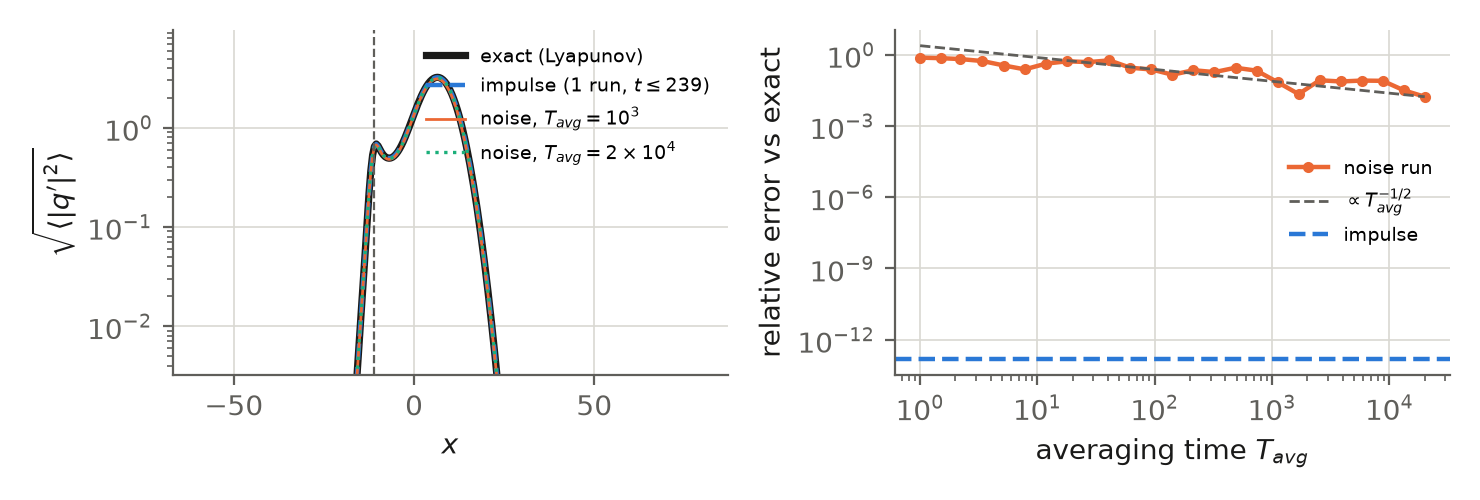
\includegraphics[width=0.74\linewidth]{Images/gl_rank1.png}
	\end{center}
	\vspace{-0.2cm}
	\begin{itemize}
		\item Exact $C$ from the discrete Lyapunov equation. Impulse (one run, $t\le239$): error $1.5\times10^{-13}$. Noise run: error $1.7\times10^{-2}$ after $T_{avg}=2\times10^4$, decreasing as $T_{avg}^{-1/2}$.
	\end{itemize}
\end{frame}

%----------------------------------------------------------------------
\begin{frame}
	\frametitle{Demonstration on a model problem: noise at every point}
	\footnotesize
	Same model, forcing $f_j=g(x_j)\,\xi_j(t)$ with an independent signal at each of the 15 grid points inside the Gaussian (like \texttt{awgn} per quadrature point).
	\begin{center}
		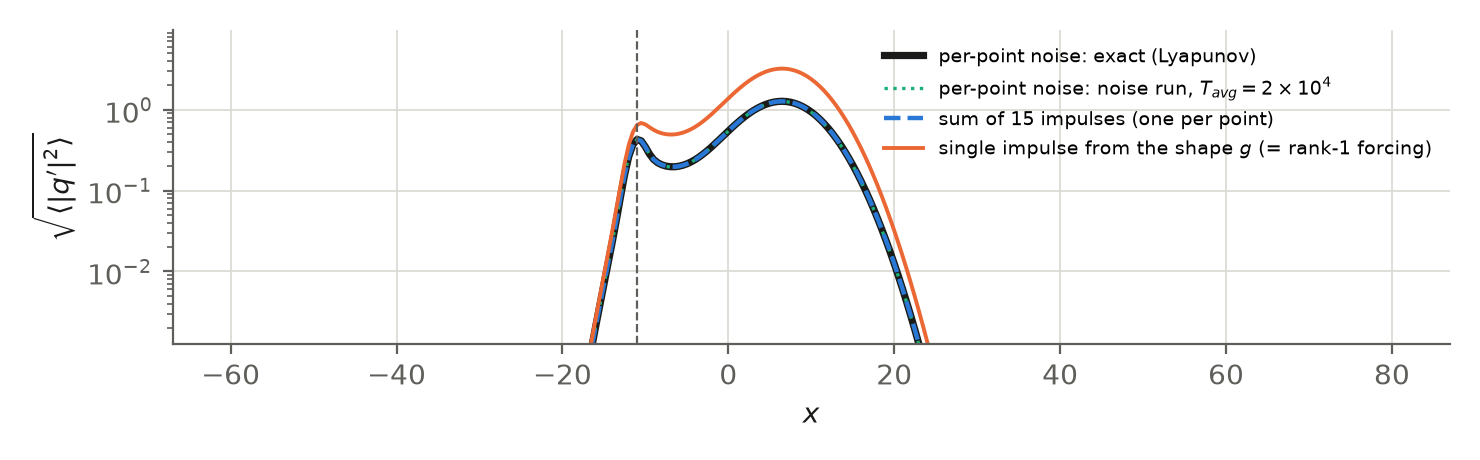
\includegraphics[width=0.74\linewidth]{Images/gl_perpoint.png}
	\end{center}
	\vspace{-0.2cm}
	\begin{itemize}
		\item Sum of 15 impulse runs (one per point): error $1.5\times10^{-13}$. Noise run: $0.9\times10^{-2}$.
		\item A single impulse from the shape $g$ (the rank-1 forcing) is a different forcing: level $6.4\times$ higher here, because the 15 sources add coherently instead of incoherently. Downstream of the forcing the normalised shapes agree within $0.2\%$: the Gaussian is narrow compared with the wavelength, so here the two forcings differ by a constant factor only (not guaranteed in general).
	\end{itemize}
\end{frame}

%----------------------------------------------------------------------
\begin{frame}
	\frametitle{What this means for the gap study}
	\small
	\begin{itemize}
		\item The impulse run is not an approximation of the noise run: for a rank-1 white-noise forcing both compute the same covariance, the impulse run without statistical error and in one transit time.
		\item Matching the existing incompressible averages requires the same forcing: either per-point noise ($m$ impulse runs, $m$ mesh dependent), or redo the incompressible reference with the rank-1 dipole (an incompressible impulse run took 77 min).
		\item Levels scale with $\sigma^2$ (forcing amplitude squared, times $\Delta t$ for per-step noise); shapes, $N$ factors and ratios between geometries or Mach numbers do not depend on it.
		\item The same impulse response also gives the spectra: $S_{uu}(\mathbf{x},\omega)=\sigma^2|\hat u_h(\mathbf{x},\omega)|^2$ (FFT of the impulse response), i.e.\ which frequencies are amplified where.
	\end{itemize}
\end{frame}

%----------------------------------------------------------------------
\begin{frame}
	\frametitle{Impulse runs on the HPC}
	\small
	\begin{itemize}
		\item Settings: $\Delta t=0.2$, $T=28$, $\delta=10^{-6}$, samples every 1.4, $t\in[0,3640]$, 32 cores (one node).
		\item Wall time: \textbf{30--70 min per case} on the DNS meshes, 6.7 h on the incompressible mesh (4000 elements, $P=5$), vs days for a noise run with long averaging.
		\item Converged: $\int u'^2dt$ changes by $3\times10^{-4}$ between $t=2912$ and $3640$ ($3\times10^{-3}$ for $x>600$).
	\end{itemize}
	\begin{center}
		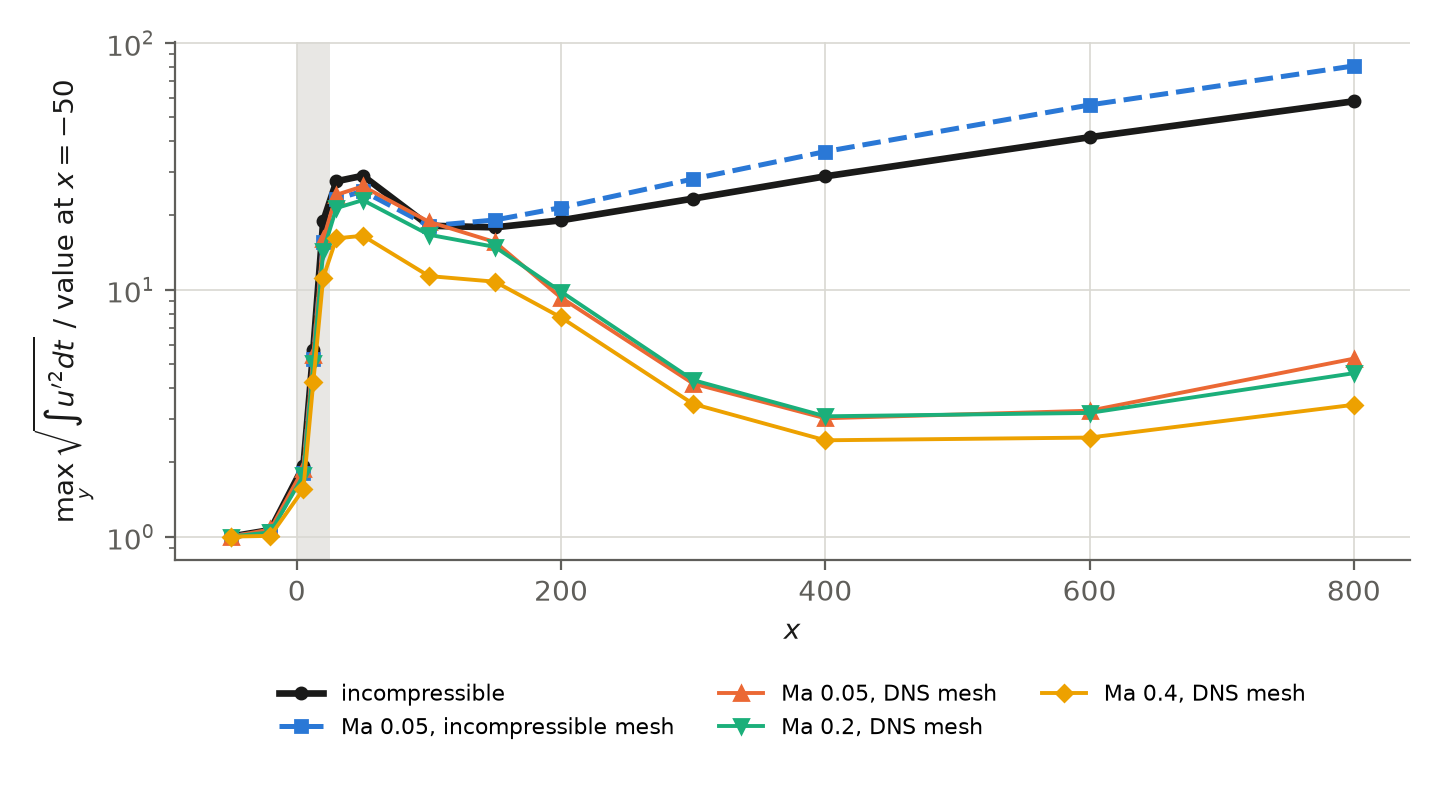
\includegraphics[width=0.52\linewidth]{Images/impulse_growth.png}
	\end{center}
\end{frame}

%----------------------------------------------------------------------
\begin{frame}
	\frametitle{Compressible vs incompressible: the mesh matters downstream}
	\begin{columns}[T]
		\begin{column}{0.56\linewidth}
			\centering
			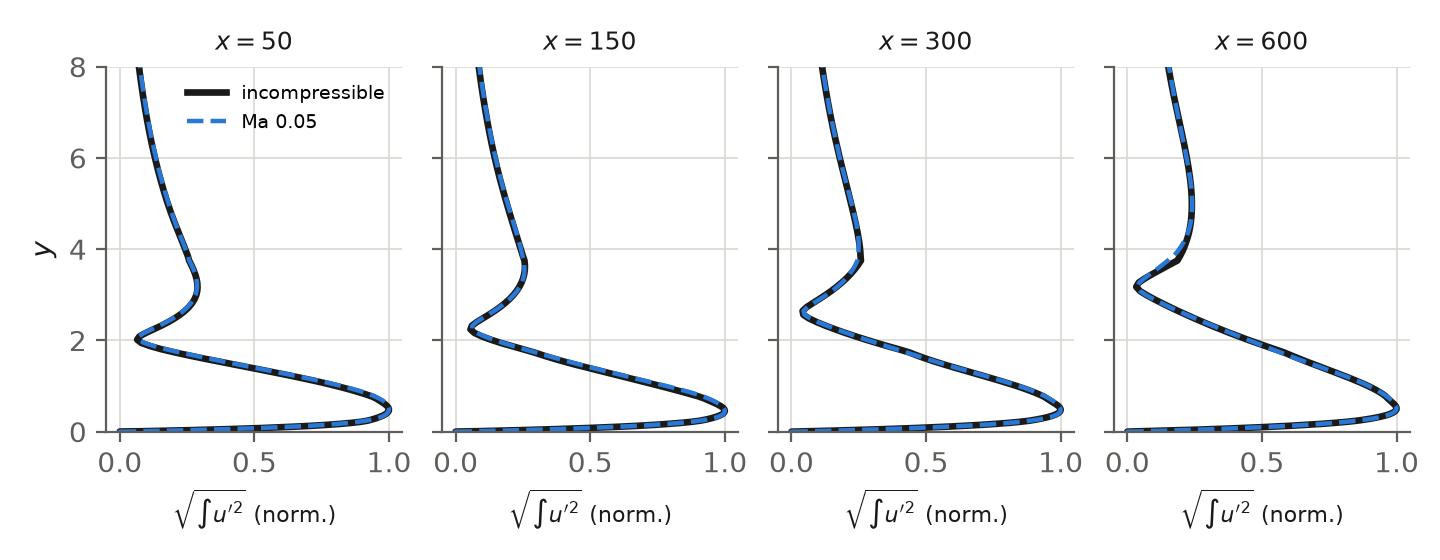
\includegraphics[width=\linewidth]{Images/impulse_profiles.png}\par\vspace{0.15cm}
			{\footnotesize Same mesh (incompressible case), Ma 0.05: the normalised\\ wall-normal profiles agree within 1--2\%.}
		\end{column}
		\begin{column}{0.42\linewidth}
			\footnotesize
			\begin{itemize}
				\item On the same mesh: receptivity identical (0.4\% at $x=-50$), gap within 18\%, TS growth downstream present, $\sim35\%$ more by $x=600$ (growth rate difference $\sim2\times10^{-4}$: SVV of the incompressible run, base flow not an exact compressible steady state).
				\item On the compressible DNS meshes: the packet \emph{decays} for $x>150$ at every Mach number.
				\item Cause: the DNS meshes cap the horizontal element size per layer, $h_{\max}=\{8,10,20,50,100,\dots\}$; TS waves of wavelength 20--35 living up to $y\approx3$--$5$ get $\sim1$ element per wavelength at $P=4$. Fine for the (smooth) steady state, not for travelling waves.
				\item Upstream and over the gap ($x\le100$) the DNS-mesh results are usable: more stable with Mach.
			\end{itemize}
		\end{column}
	\end{columns}
\end{frame}

%----------------------------------------------------------------------
\begin{frame}
	\frametitle{Refined DNS mesh: the downstream growth is recovered}
	\small
	Ma 0.05, d1.5\_w25, DNS steady state interpolated onto the refined meshes (drift $6\times10^{-6}$ per period). $A(x)=\max_y\sqrt{\int u'^2dt}$:
	\begin{center}\footnotesize
		\renewcommand{\arraystretch}{1.1}
		\begin{tabular}{rcccccc}
			\toprule
			$x$ & incompressible & Ma 0.05, incomp.\ mesh & DNS mesh & R1 & R2 & R1/R2 \\
			\midrule
			$-50$ & 0.466 & 0.464 & 0.771 & 0.483 & 0.454 & 1.06 \\
			20    & 8.83  & 7.22  & 12.3  & 7.61  & 7.17  & 1.06 \\
			100   & 8.46  & 8.42  & 14.5  & 9.15  & 8.51  & 1.08 \\
			300   & 10.9  & 13.0  & 3.2   & 13.6  & 12.7  & 1.07 \\
			600   & 19.3  & 26.0  & 2.5   & 26.0  & 24.8  & 1.05 \\
			800   & 27.0  & 37.4  & 4.1   & 37.8  & 36.8  & 1.03 \\
			\bottomrule
		\end{tabular}
	\end{center}
	\begin{itemize}\footnotesize
		\item R1 ($h_{\max}=\{4,4,4,5,8,20,50,200\}$, 1955 quads, 2.0 h) and R2 ($\{2,2,2,3,5,10,30,100\}$, 3225 quads, 5.4 h): same growth (constant ratio, profile shapes within 0.2\%), and both match the run on the incompressible mesh downstream.
		\item The constant $\sim6\%$ offset comes from the receptivity at the forcing ($x_0=-95$): only absolute levels, not $N$ factors. A local refinement around $x_0$ would remove it.
	\end{itemize}
\end{frame}

%----------------------------------------------------------------------
\begin{frame}
	\frametitle{Batch: refined meshes for all the steady base flows}
	\small
	\begin{itemize}
		\item 94 cases with a steady DNS base flow ($\max|\Delta u|<10^{-6}$ over the last $\ge150$ time units): Ma 0.05 (23), 0.2 (21), 0.4 (20), 0.6 (15), 0.8 (15).
		\item Same \texttt{mesh.geo} with $h_{\max}=\{4,4,4,5,8,20,50,200\}$ (R1, 1955 vs 1074 quads); the job interpolates the DNS steady state onto the refined mesh (same geometry) and runs the impulse response.
		\item Prepared in \texttt{comGapRe1000Ma*/directLinearSolver/blowingSuction/<case>/}; submission with \texttt{pp\_submit\_impulse.sh [Ma \dots]}.
		\item R1 checked on Ma 0.05, d1.5\_w25 against R2 and the incompressible mesh (previous slide): 2.0 h per case on one node.
	\end{itemize}
	\vspace{0.2cm}
	\textbf{Questions}
	\begin{itemize}
		\item Forcing model for the study: impulse (coherent dipole $\times$ white noise) instead of per-point noise? Absolute levels are not comparable with the earlier incompressible averages; shapes and $N$ factors are.
		\item Resolved dipole (\texttt{weight} = 1) for all the cases?
	\end{itemize}
\end{frame}

\end{document}
